\subsection{sacabench construct}
\label{framework:cli:sacabench-construct}

{
\begin{wrapfigure}[30]{R}[5mm]{.5\textwidth}
    \vspace{-1.5\baselineskip}
    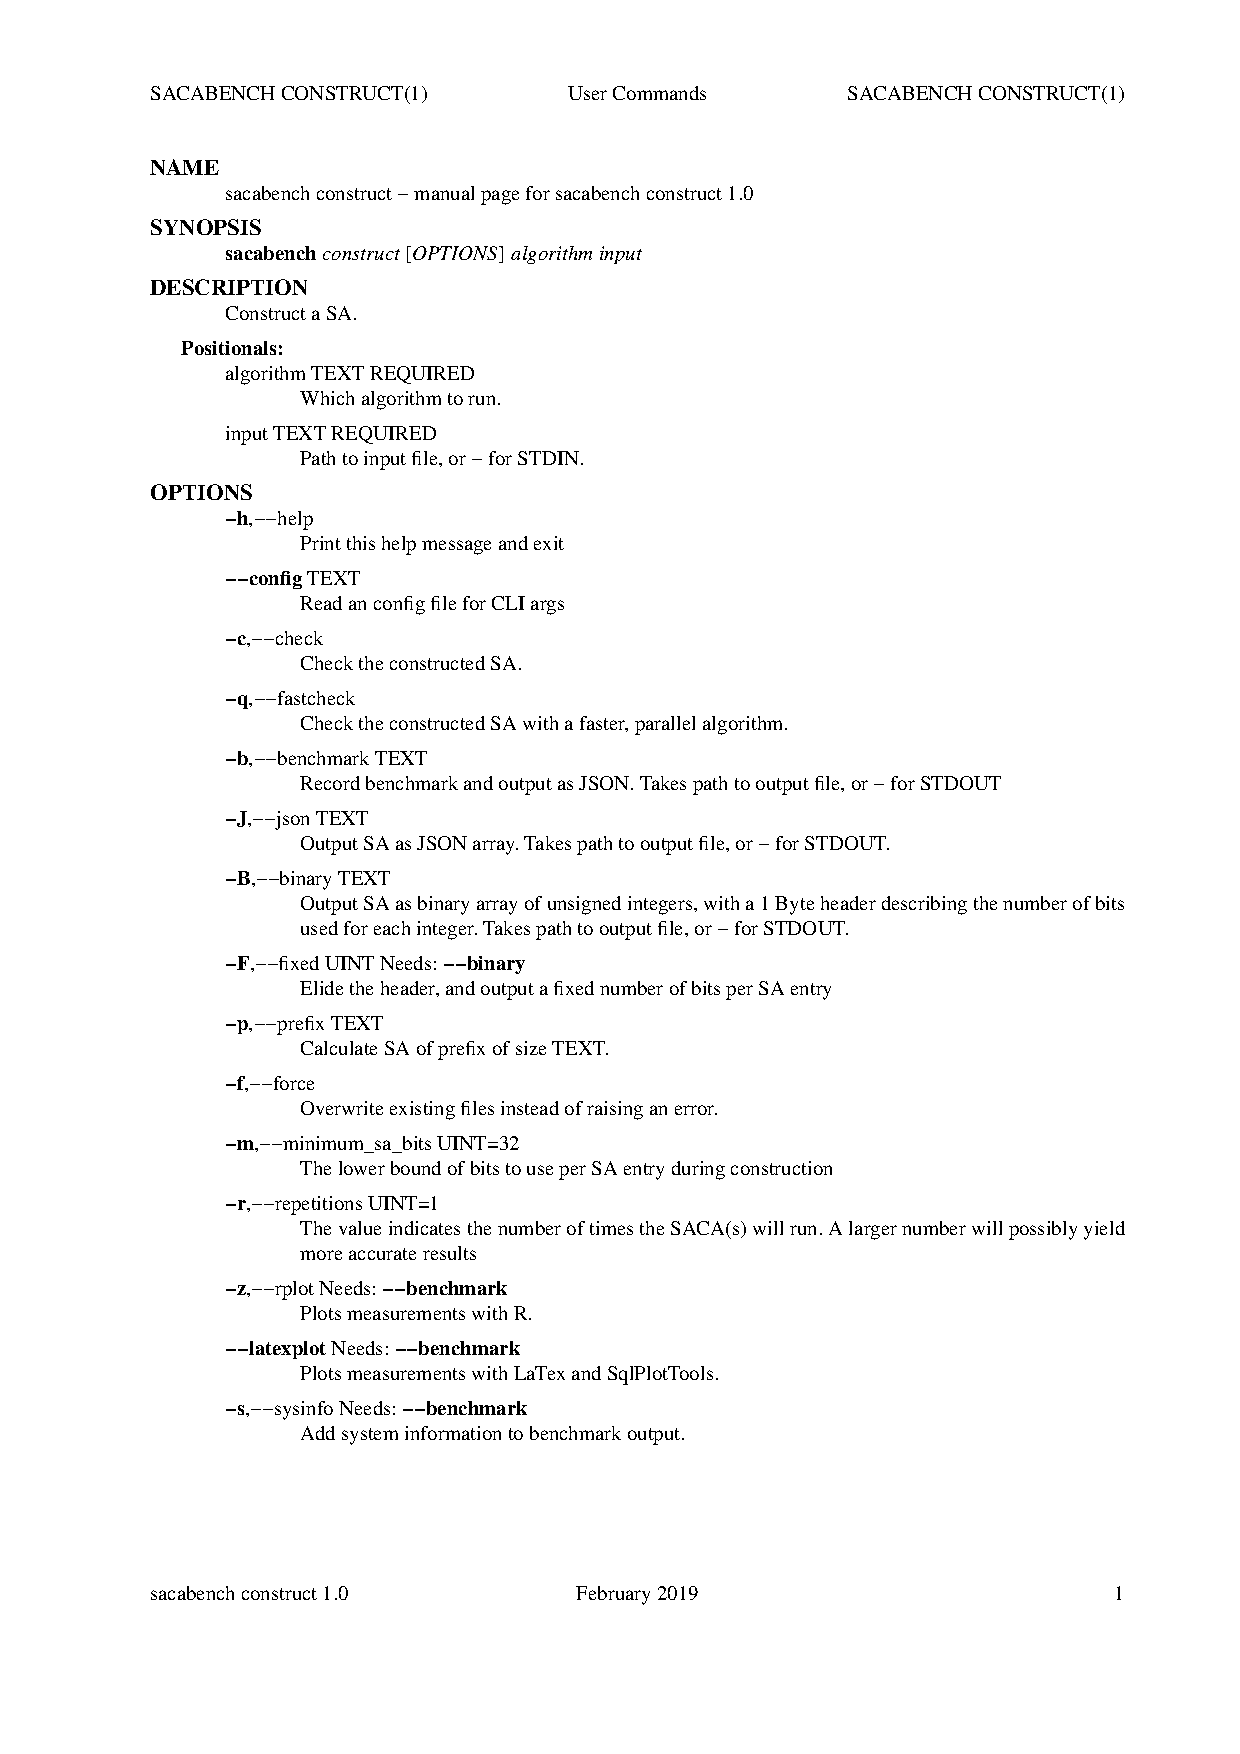
\includegraphics[page=1, viewport=0cm 32.8cm 20.5cm 68.5cm, clip, width=.5\textwidth]{{kapitel/3_framework/cli/sacabench-construct/sacabench-construct}.pdf}\\
    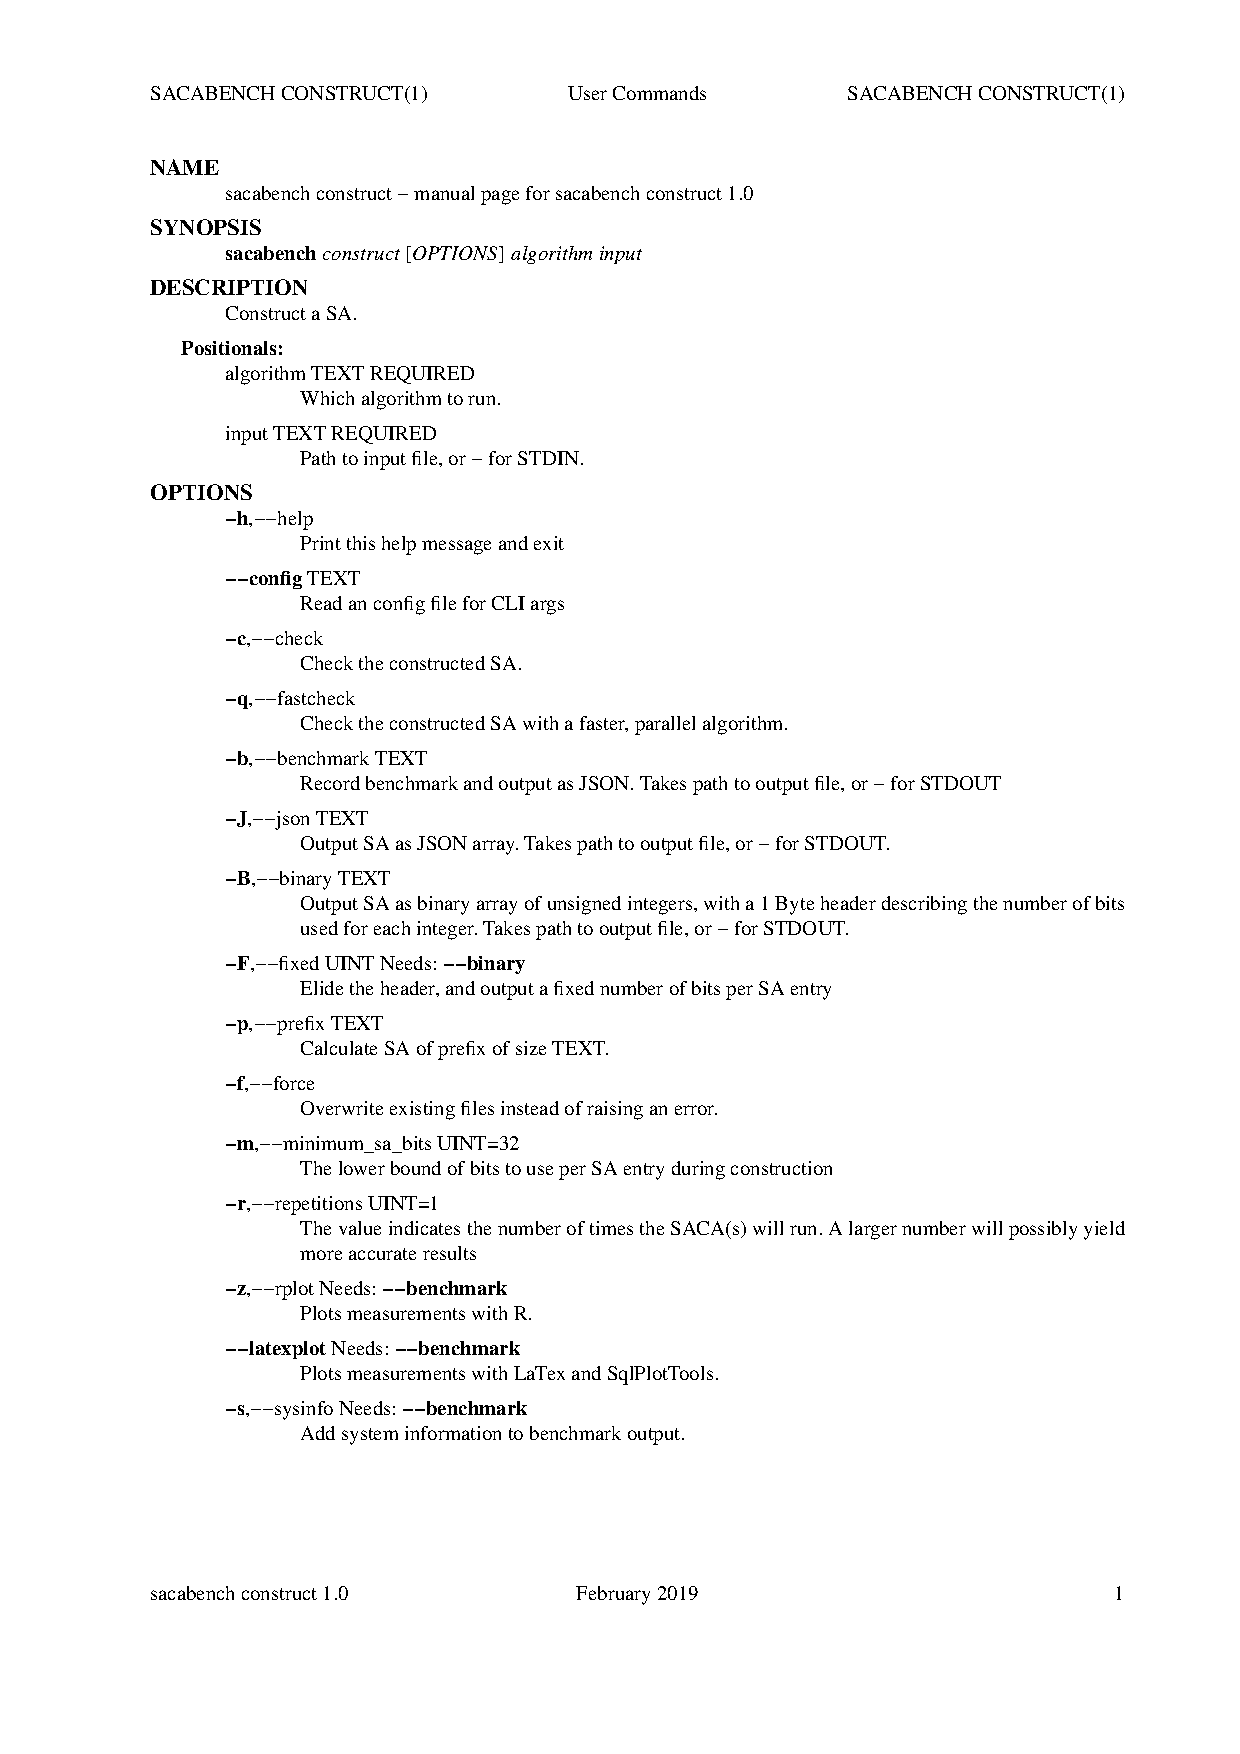
\includegraphics[page=1, viewport=0cm 25cm 20.5cm 26.3cm, clip, width=.5\textwidth]{{kapitel/3_framework/cli/sacabench-construct/sacabench-construct}.pdf}\\
    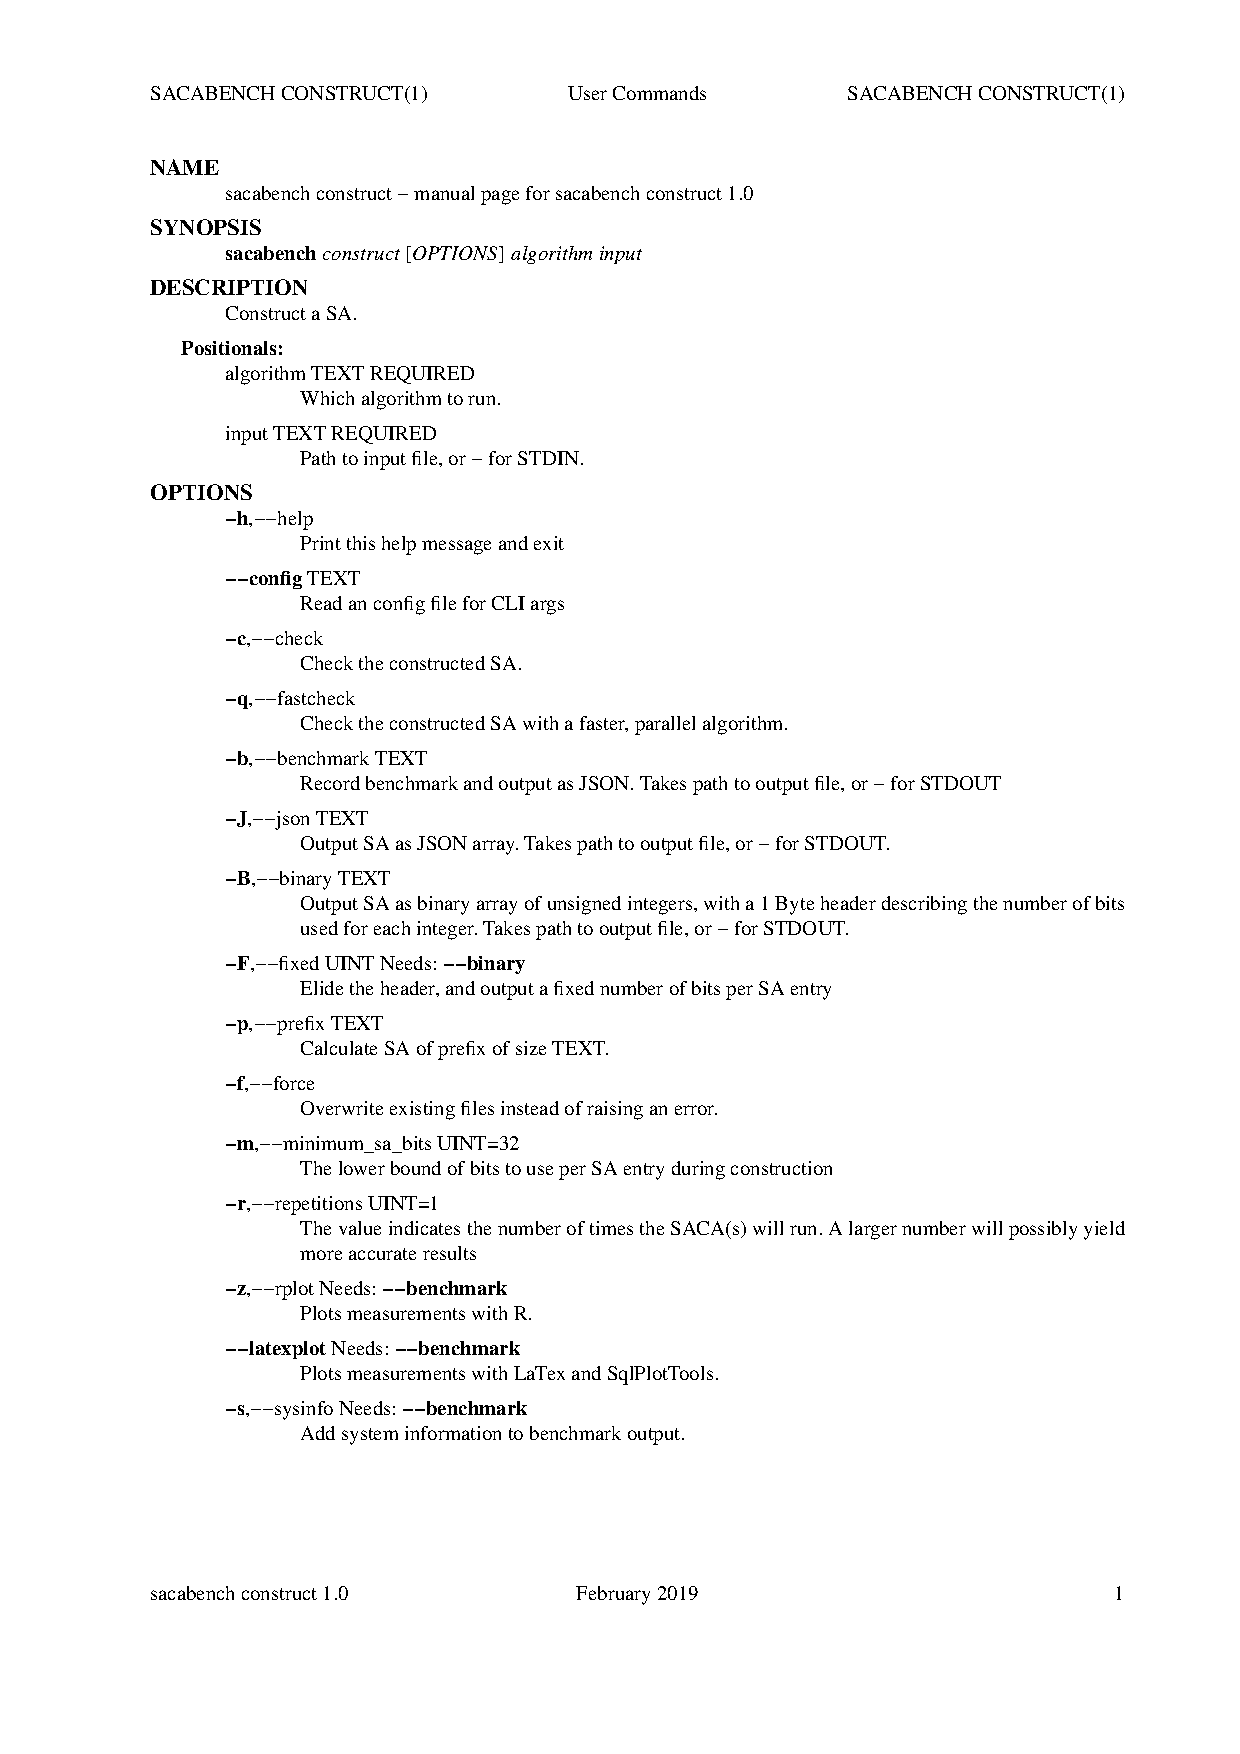
\includegraphics[page=1, viewport=0cm 0cm 20.5cm 1.5cm, clip, width=.5\textwidth]{{kapitel/3_framework/cli/sacabench-construct/sacabench-construct}.pdf}
    \caption{gekürzte Ausgabe von \texttt{man sacabench construct}}
    \label{manpage:sacabench-construct}
\end{wrapfigure}

Mit dem Befehl \texttt{sacabench construct} kann ein ausgewählter Algorithmus ausgeführt werden. 
\par
Der auszuf{\"u}hrende Algorithmus wird dabei durch sein K{\"u}rzel bestimmt, wie es bei \termfont{sacabench list} angegeben ist. 
Gefolgt wird der Name des Algorithmus durch den Text, auf den er angewendet werden soll. 
Hierf{\"u}r kann ein Pfad zu einer Textdatei oder alternativ \termfont{-} f{\"u}r STDIN angegeben werden. 
\par
Zus{\"a}tzlich kann eine ganze Reihe von Optionen angegeben werden. 
Wie auch bei anderen Subcommands zeigen \termfont{-h} und \termfont{-{}-help} die Hilfe an. 
Die Option \termfont{-c} bzw. \termfont{-{}-check} wendet zus{\"a}tzlich zu dem ausgew{\"a}hlten Algorithmus einen weiteren SACA auf die Eingabe an und {\"u}berpr{\"u}ft, ob die beiden Ergebnisse gleich sind. 
Ist dies nicht der Fall, wird eine Fehlermeldung angezeigt. 
Wird die Option \termfont{-b} oder \termfont{-{}-benchmark} gefolgt von einem Pfad angegeben, wird an diesem Pfad eine JSON-Datei mit den gemessenen Zeiten und Speicherverbrauch angelegt. 
Existiert an dem angegebenen Pfad bereits eine Datei, kann diese mit der Option \termfont{-f} bzw. \termfont{-{}-force} {\"u}berschrieben und durch die neue Messung ersetzt werden. 
Der Inhalt dieser Datei ist die Grundlage f{\"u}r die erstellten Diagramme, welche mit \termfont{-z} oder \termfont{-{}-plot} bei der Ausf{\"u}hrung des Algorithmus generiert werden. 
Um bei den Messungen ein besseres Ergebnis zu erhalten, kann mit der Option \termfont{-r} bzw. \termfont{-{}-repetitions} eine Anzahl an Durchf{\"u}hrungen festgelegt werden. 
Hierdurch wird die Genauigkeit der Messung erh{\"o}ht, indem das Arithmetische Mittel gebildet wird.
Weiterhin kann dem Befehl \termfont{-p} oder \termfont{-{}-prefix} hinzugef{\"u}gt werden. 
Hierbei kann die Anzahl an f{\"u}hrenden Bytes angegeben werden, die von der Eingabe verarbeitet werden sollen.
Um gr{\"o}{\ss}ere Werte leichter angeben zu k{\"o}nnen, sind die Abk{\"u}rzenden Schreibweisen K und M erlaubt, welche f{\"u}r Kilobyte bzw. Megabyte stehen.
Dies sorgt daf{\"u}r, dass von der {\"u}bergebenen Textdatei nur so viele Bytes verarbeitet werden, wie durch diese Option angegeben werden. 
Die Option \termfont{-B} oder \termfont{-{}-binary} veranlasst das Framework zur Ausgabe in bin{\"a}rer Form.
Anschlie{\ss}end werden die Eintr{\"a}ge des Ergebnisses als Bin{\"a}rzahlen mit bis zu 8 Stellen ausgegeben. 
Die erste Zahl der Ausgabe gibt die genaue Anzahl der Stellen an.
Ist eine feste Anzahl an Bits gew{\"u}nscht, kann diese mit der Option \termfont{-F} bzw. \termfont{-{}-fixed} angegeben werden.
Die letzte Option, welche dem Subcommand \texttt{sacabench construct} {\"u}bergeben werden kann, ist \termfont{-m} oder \termfont{-{}-minimum\_sa\_bits} gefolgt von einem UINT Wert. Dieser Parameter bestimmt die Anzahl der Bits, die f{\"u}r die Datenstrukturen w{\"a}hrend der Berechnung genutzt werden.
\par
}
